\documentclass[Rapport/Rapport_main.tex]{subfiles}
\begin{document}
\section{Metode og proces}
\subsection{Introduktion}
I dette afsnit beskrives processen af et 3. semester projekt omhandlende udviklingen af et interaktivt Beer Pong bord. Derfor er dette afsnit en opsummering af bilage \textbf{Proces}. Udover processen vil der også være en beskrivelse af de metoder og redskaber, der er blevet anvendt under forløbet. \\
Som det første er det værd at kigge på de krav der er for processen i forbindelse med 3. semester projektet\cite{Universitet2018}. De to krav, der har med processen at gøre er \textit{"Anvendelsen af processer og metoder kendt fra projektet på 2. semester, men anvendt iterativt over alle faser."} og \textit{"Iterativ arbejdsmetode, SCRUM, orienteret mod at udvikle nye produkter baseret på HW og SW."}. Det er helt tydeligt her at dette projekt skal udvikles iterativ gennem Scrum, og derfor vil det næste under afsnit fokusere på det.

\subsection{Andvendelse af Scrum i PRJ3, Gruppe7}
Som sagt er dette afsnit dedikeret til at beskrive den anvendelse af Scrum, der har været for Gruppe7. Gennem den proces der har været i forbindelse med projektet, er der blevet gjort mange forskellige erfaringer i forhold til, hvad der har fungeret for netop Gruppe7. Til at starte med er det værd at vise den overordnede skitse, der er blevet lavet til at beskrive, hvordan der anvendes Scrum i netop Gruppe7. Denne kan ses i figur \ref{fig:rap_scrum_usage}.
\begin{figure}[H]
    \centering
    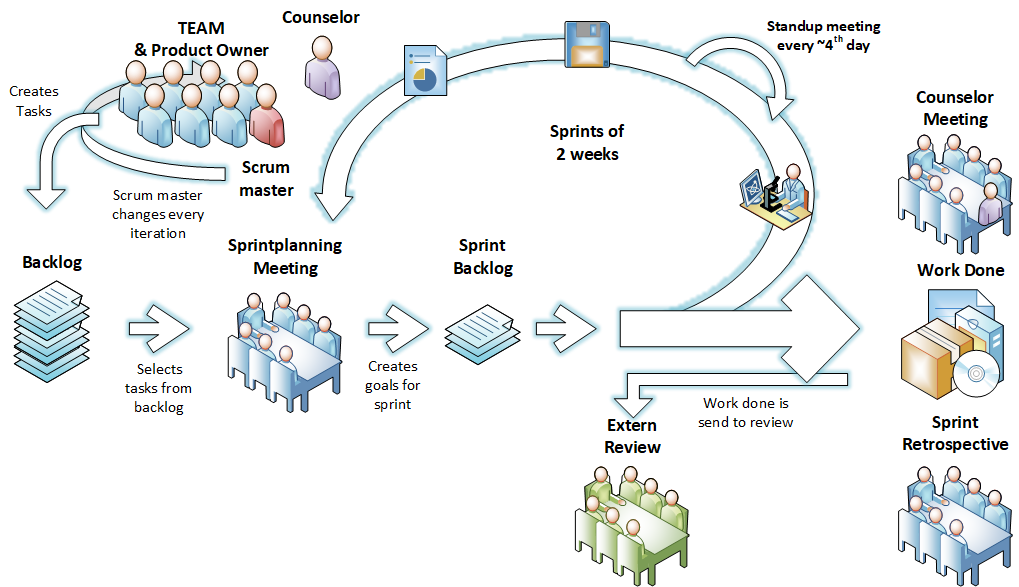
\includegraphics[width=\textwidth]{Processdokument/graphics/Scrum_usage.png}
    \caption{Gruppens skitse for hvordan der er anvendt SCRUM i projektet}
    \label{fig:rap_scrum_usage}
\end{figure}
Af figur \ref{fig:rap_scrum_usage} ses det i øverste venstre hjørne, hvordan gruppen selv har varetaget rollen som Product Owner, da det er deres projekt, der udvikles og de bestemmer hvilke funktioner og egenskaber, der skal prioriteres i deres projekt. Samme sted ses det også, hvordan rollen som Scrum Master er gået på tur efter hvert sprint, da alle skulle prøve at have ansvaret og erfaringerne, der følger med rollen. I midten af venstre side ses det, hvordan der til Sprint-planlægningsmøder er blevet udvalgt de relevante tasks fra backloggen til at have med i det nye sprint. Hertil laves en sprint backlog, der indeholder alle tasks i sprintet. Der var desuden gode erfaringer med at sætte konkrete målbare mål i sprintplanlægningen. Det kunne for eksempel være at have demoer klar til vejleder møde eller dokumenter færdiggjort.\\
Efter at sprintet af planlagt udføres et sprint på 2 ugers tid, hvor der undervejs i sprintet laves Standup Meetings, på de dage hvor det aftaltes at mødes. Til disse møder opdateres hele teamet i forhold til, hvor langt de enkelte er med deres opgaver, og om der er problemer eller mangler hjælp et sted.\\
Til slut i sprintet laves så et møde med vejleder, hvor der evalueres Risikoer i forbindelse med projektet, så der kan planlægges ud fra disse. Desuden stilles der forskellige spørgsmål i forbindelse med usikkerheder eller problemer i projektet. Efter et sprint er der selvfølgelig også arbejde, der kan være dokumentation, design eller implementation, som sendes til et eksternt review hos en anden 3. semesterprojekt gruppe. Til sidst laves et retrospektiv på Sprintet, hvor der bliver nedskrevet positive og negative ting, der har været i det pågældende sprint. Der opsættes så to-tre af de negative punkter, der er fokus på at forbedre i det næste sprint. Aktionspunkterne fra forrige Sprint blev også taget op for at se om, der rent faktisk var sket en forbedring.\\
Til at gøre Scrum meget nemmere er der blevet anvendt Redmine som værktøj til at facillitere Scrum. Redmine indeholder netop de relevante redskaber i forhold til Sprint board, oversigt over tasks, backlog og så videre. Desuden har Redmine en Wiki funktion, der blev anvendt af Scrum master til at nedskrive information omkring planlægning og retrospektiv.\\
Hvis der er interesse for anvendelsen af Scrum, samt de erfaringer, der er gjort i løbet af sprintet, så henvises der til \fullref{proces:sec:experiences_w_scrum}.

\subsection{Iterativ ASE-udviklingsmodel og SYSML}
Som krav for 3. semester projektet var der, at der skulle anvendes metoder og processer, som blev anvendt til 2. semester projektet. På 2. semester blev der til udvikling anvendt ASE-udviklingsmodellen, der kan ses på figur \ref{fig:rap_ase_model}.
\begin{figure}[H]
    \centering
    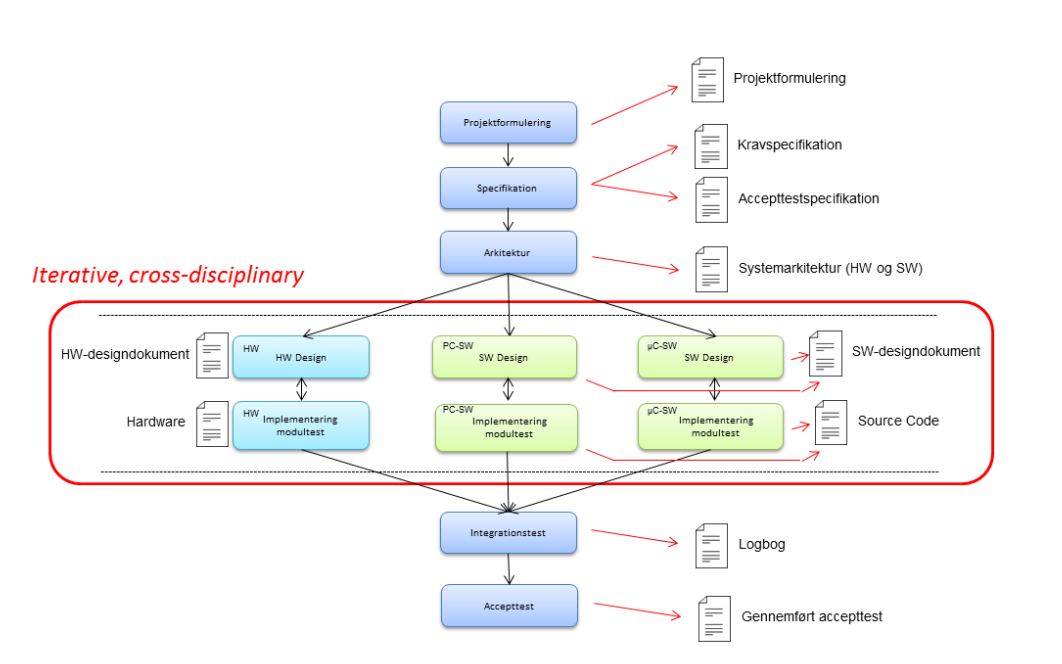
\includegraphics[width=\textwidth]{Processdokument/graphics/ASE_model.png}
    \caption{Udviklingsmodel fra ASE [Kilde: Kim Bjerge, Vejledning til udviklingsprocessen for projekt 2\cite{}]}
    \label{fig:rap_ase_model}
\end{figure}
ASE-modellen i figur \ref{fig:rap_ase_model}, blev anvendt iterativt, som det også fremgår af figuren, i Design og Implementeringsfasen. Det vil altså siges at hardware og software blev designet og implementeret iterativt. Mange af dokumenterne blev også udarbejdet iterativt, idet de i løbet af sprintene hele tiden blev forbedret og rettet.\\\\
Derudover blev der også anvendt SysML, som redskab til at modelere og beskrive systemet. I SysML blev der anvendt de begreber og metoder, der er stiftet bekendskab med i 2. semester kurset Indledende System Engineering (ISE). De anvendte SysML metoder kan ses i figur \ref{fig:rap_sysml_usage}.
\begin{figure}[H]
    \centering
    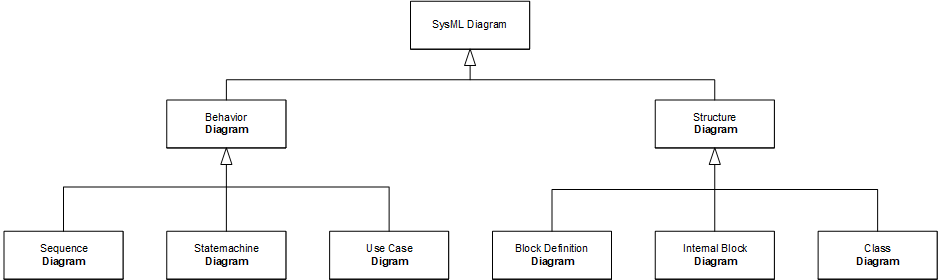
\includegraphics[width=\textwidth]{Processdokument/graphics/Sysml_usage.png}
    \caption{SysML blokke der blev anvendt i Gruppe 7}
    \label{fig:rap_sysml_usage}
\end{figure}
Af figur \ref{fig:rap_sysml_usage} ses det at opførelsen af systemet beskrives gennem Sekvens-, Statemachine- og Use Case-diagrammer.
Strukturen af systemet beskrives ved Block Definition- og Internal Block-diagram. Her er Class-Diagram inkluderet fra UML, da den beskriver strukturen og relationerne i software.

\end{document}